%% ============================================================
%%  PyBNCore — Technical Library Report
%%  Author: Akram Batikh <asbatikh@ncsu.edu>
%%  Purpose: Post-doc introduction document
%% ============================================================
\documentclass[11pt, letterpaper]{article}

% ── Packages ──────────────────────────────────────────────────────────────────
\usepackage[T1]{fontenc}
\usepackage[utf8]{inputenc}
\usepackage{lmodern}
\usepackage[margin=1in]{geometry}
\usepackage{amsmath, amssymb, amsthm}
\usepackage{algorithm}
\usepackage[noend]{algpseudocode}
\usepackage{graphicx}
\usepackage{tikz}
\usetikzlibrary{arrows.meta, positioning, shapes.geometric, fit, backgrounds, calc}
\usepackage{pgfplots}
\pgfplotsset{compat=1.18}
\usepackage{booktabs}
\usepackage{multirow}
\usepackage{listings}
\usepackage[dvipsnames]{xcolor}
\usepackage{hyperref}
\usepackage{microtype}
\usepackage{caption}
\usepackage{subcaption}
\usepackage{enumitem}
\usepackage{fancyhdr}
\usepackage{abstract}
\usepackage{titlesec}
\usepackage{cleveref}

% ── Hyperref setup ─────────────────────────────────────────────────────────────
\hypersetup{
  colorlinks = true,
  linkcolor  = NavyBlue,
  citecolor  = ForestGreen,
  urlcolor   = RoyalBlue,
  pdftitle   = {PyBNCore: A High-Performance Bayesian Network Inference Engine},
  pdfauthor  = {Akram Batikh},
}

% ── Code listing style ──────────────────────────────────────────────────────────
\lstdefinestyle{cppstyle}{
  language        = C++,
  basicstyle      = \ttfamily\small,
  keywordstyle    = \color{NavyBlue}\bfseries,
  commentstyle    = \color{ForestGreen}\itshape,
  stringstyle     = \color{BrickRed},
  numbers         = left,
  numberstyle     = \tiny\color{gray},
  breaklines      = true,
  showstringspaces= false,
  frame           = single,
  rulecolor       = \color{gray!40},
  backgroundcolor = \color{gray!5},
  tabsize         = 2,
  captionpos      = b,
}
\lstdefinestyle{pythonstyle}{
  language        = Python,
  basicstyle      = \ttfamily\small,
  keywordstyle    = \color{NavyBlue}\bfseries,
  commentstyle    = \color{ForestGreen}\itshape,
  stringstyle     = \color{BrickRed},
  numbers         = left,
  numberstyle     = \tiny\color{gray},
  breaklines      = true,
  showstringspaces= false,
  frame           = single,
  rulecolor       = \color{gray!40},
  backgroundcolor = \color{gray!5},
  captionpos      = b,
}

% ── Header / footer ─────────────────────────────────────────────────────────────
\pagestyle{fancy}
\fancyhf{}
\lhead{\small PyBNCore — Technical Report}
\rhead{\small Akram Batikh, NC State University}
\cfoot{\thepage}
\renewcommand{\headrulewidth}{0.4pt}

% ── Section title formatting ─────────────────────────────────────────────────────
\titleformat{\section}{\large\bfseries}{{\color{NavyBlue}\thesection}}{1em}{}[\vspace{-2pt}\rule{\linewidth}{0.4pt}]
\titleformat{\subsection}{\normalsize\bfseries}{{\color{NavyBlue}\thesubsection}}{1em}{}

% ── Custom commands ──────────────────────────────────────────────────────────────
\newcommand{\bncore}{\textsc{PyBNCore}}
\newcommand{\smiletool}{\textsc{SMILE}}
\newcommand{\R}{\mathbb{R}}
\newcommand{\E}{\mathbb{E}}
\newcommand{\Pa}{\mathrm{Pa}}
\newcommand{\scope}{\mathrm{scope}}
\newtheoremstyle{definitionstyle}{6pt}{6pt}{\itshape}{}{\bfseries\color{NavyBlue}}{.}{.5em}{}
\theoremstyle{definitionstyle}
\newtheorem{definition}{Definition}
\newtheorem{theorem}{Theorem}

% ══════════════════════════════════════════════════════════════════════════════
\begin{document}

% ── Title page ─────────────────────────────────────────────────────────────────
\begin{titlepage}
  \centering
  \vspace*{1.5cm}
  {\huge\bfseries \bncore{}\par}
  \vspace{0.5cm}
  {\large\itshape A High-Performance C++/Python Bayesian Network\\
  Inference Engine for Probabilistic Risk Analysis\par}
  \vspace{2cm}
  \rule{\linewidth}{0.5pt}\\[0.5em]
  {\normalsize
    \textbf{Akram Batikh}\\
    Department of Nuclear Engineering\\
    North Carolina State University\\
    \href{mailto:asbatikh@ncsu.edu}{asbatikh@ncsu.edu}
  }\\[0.5em]
  \rule{\linewidth}{0.5pt}
  \vspace{1cm}

  \begin{abstract}
    \noindent
    \bncore{} is an open-source, high-performance Bayesian Network (BN)
    inference engine designed for large-scale Monte Carlo and epistemic
    uncertainty analyses in Probabilistic Risk Assessment (PRA). The
    library provides a C++17 backend with zero-allocation inference
    kernels, SIMD-accelerated factor arithmetic, and multi-threaded
    batched execution, exposed through idiomatic Python bindings via
    \texttt{nanobind}. Unlike commercial tools such as \smiletool{}/GeNIe,
    which execute one scenario at a time, \bncore{} ingests an entire
    \emph{batch} of evidence scenarios as a NumPy matrix and solves them
    simultaneously, achieving speedups of up to two orders of magnitude on
    million-scenario workloads. The engine implements exact Shafer--Shenoy
    belief propagation on Junction Trees compiled via moralization,
    triangulation (weighted min-fill heuristic), and Kruskal's maximum
    spanning tree algorithm. Additional capabilities include soft/virtual
    evidence, MAP/MPE inference with traceback, parameter sensitivity
    analysis, and Value of Information ranking.
  \end{abstract}

  \vfill
  {\small Version 1.0 \quad \today}
\end{titlepage}

% ── Table of contents ───────────────────────────────────────────────────────────
\tableofcontents
\newpage

% ══════════════════════════════════════════════════════════════════════════════
\section{Motivation and Background}
\label{sec:motivation}
% ══════════════════════════════════════════════════════════════════════════════

Probabilistic Risk Assessment (PRA) models for nuclear power plants
routinely embed hundreds of Bayesian Networks (BNs) that encode causal
relationships between component failures, human error probabilities
(HEPs), and system-level outcomes. A typical Level-1 multi-hazard PRA
study requires evaluating these networks over $10^5$--$10^6$ Monte Carlo
scenarios — each with a distinct evidence vector representing a sampled
system state. With existing commercial BN tools (\smiletool{}, Netica,
pgmpy), each scenario is processed sequentially, saturating a single CPU
core and rendering million-scenario epistemic sweeps impractical
($\gtrsim$hours).

\bncore{} addresses this bottleneck through a fundamentally different
execution model: the \emph{batch-major} execution paradigm. Rather than
looping over scenarios, it treats the entire scenario ensemble as an
additional tensor dimension and executes a single vectorized pass over
all scenarios simultaneously. The result is near-linear scalability with
batch size on modern multi-core hardware, with no sacrifice of exactness.

The library is structured around four interacting subsystems (see
\cref{fig:architecture}):
\begin{enumerate}[topsep=2pt, itemsep=2pt]
  \item \textbf{Graph \& Factor Layer} — DAG representation and
        probability tensor arithmetic.
  \item \textbf{Junction Tree Compiler} — One-time off-line compilation
        of the DAG into an execution-ready Clique Tree.
  \item \textbf{Batched Execution Engine} — Parallel chunked execution
        with workspace caching and GIL-free multithreading.
  \item \textbf{Python Binding Layer} — Zero-copy NumPy integration via
        \texttt{nanobind}.
\end{enumerate}


% ── Architecture figure ─────────────────────────────────────────────────────────
\begin{figure}[ht]
\centering
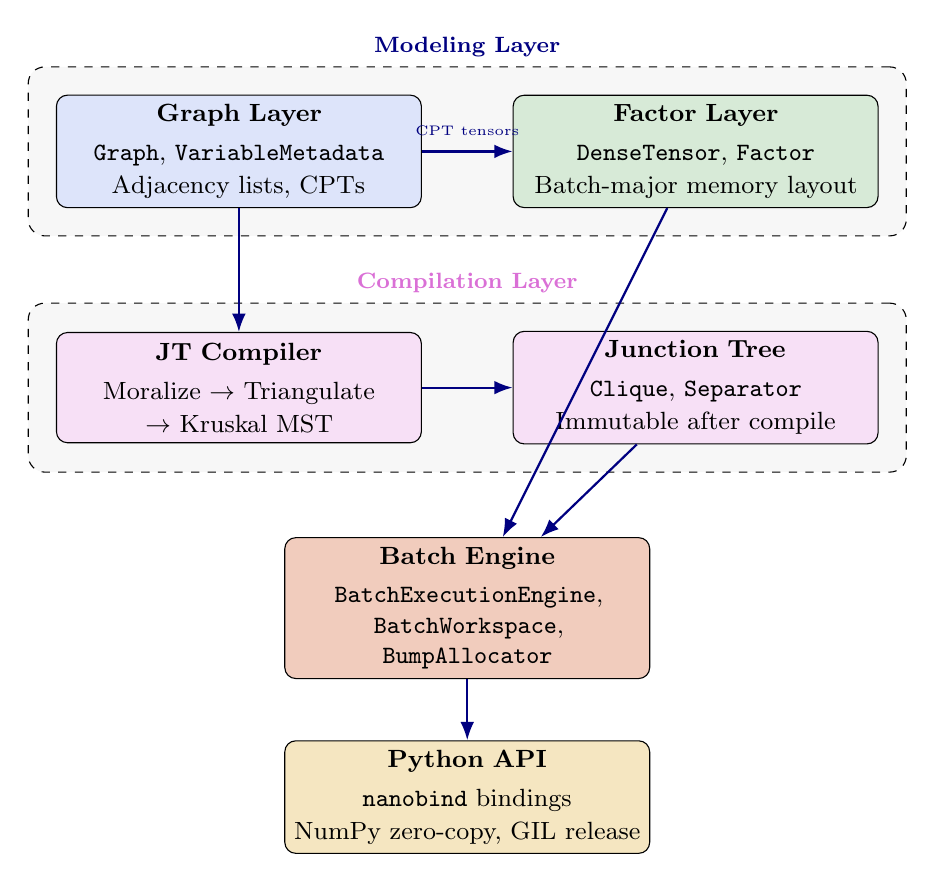
\begin{tikzpicture}[
  font         = \small,
  % Wider boxes (4.4 cm) with taller minimum height so multiline labels fit
  box/.style   = {draw, rounded corners=4pt, minimum height=1.4cm,
                  text centered, text width=4.4cm, align=center},
  layer/.style = {draw, dashed, rounded corners=6pt, inner sep=10pt,
                  fill=gray!6},
  arr/.style   = {-Latex, thick, color=NavyBlue},
]

% Column centres: left=0, right=5.8 cm.  Row centres: 0, -3.0, -5.8, -8.2
\node[box, fill=RoyalBlue!18]   (graph)    at (0, 0)
      {\textbf{Graph Layer}\\[3pt]
       \texttt{Graph}, \texttt{VariableMetadata}\\[1pt]
       Adjacency lists, CPTs};

\node[box, fill=ForestGreen!18] (factor)   at (5.8, 0)
      {\textbf{Factor Layer}\\[3pt]
       \texttt{DenseTensor}, \texttt{Factor}\\[1pt]
       Batch-major memory layout};

\node[box, fill=Orchid!22]      (compiler) at (0, -3.0)
      {\textbf{JT Compiler}\\[3pt]
       Moralize $\to$ Triangulate\\[1pt]
       $\to$ Kruskal MST};

\node[box, fill=Orchid!22]      (jt)       at (5.8, -3.0)
      {\textbf{Junction Tree}\\[3pt]
       \texttt{Clique}, \texttt{Separator}\\[1pt]
       Immutable after compile};

\node[box, fill=BrickRed!18]    (engine)   at (2.9, -5.8)
      {\textbf{Batch Engine}\\[3pt]
       \texttt{BatchExecutionEngine},
       \texttt{BatchWorkspace},
       \texttt{BumpAllocator}};

\node[box, fill=Goldenrod!28]   (python)   at (2.9, -8.2)
      {\textbf{Python API}\\[3pt]
       \texttt{nanobind} bindings\\[1pt]
       NumPy zero-copy, GIL release};

% ── Arrows ─────────────────────────────────────────────────────────────────────
\draw[arr] (graph)    -- (compiler);
\draw[arr] (factor)   -- (engine);
\draw[arr] (compiler) -- (jt);
\draw[arr] (jt)       -- (engine);
\draw[arr] (graph)    -- (factor)
           node[midway, above, font=\tiny, yshift=2pt] {CPT tensors};
\draw[arr] (engine)   -- (python);

% ── Layer brackets ─────────────────────────────────────────────────────────────
\begin{scope}[on background layer]
  \node[layer, fit=(graph)(factor),
        label={[font=\footnotesize\bfseries, color=NavyBlue]above:Modeling Layer}]
        {};
  \node[layer, fit=(compiler)(jt),
        label={[font=\footnotesize\bfseries, color=Orchid]above:Compilation Layer}]
        {};
\end{scope}

\end{tikzpicture}
\caption{High-level architecture of \bncore{}. The compile-time layer is
executed once per model; the execution layer handles every batch query.}
\label{fig:architecture}
\end{figure}


% ══════════════════════════════════════════════════════════════════════════════
\section{Probabilistic Foundations}
\label{sec:foundations}
% ══════════════════════════════════════════════════════════════════════════════

\begin{definition}[Bayesian Network]
A Bayesian Network is a tuple $\mathcal{B} = (\mathcal{G},\, \Theta)$
where $\mathcal{G} = (\mathcal{V}, \mathcal{E})$ is a Directed Acyclic
Graph (DAG) over random variables $X_1, \ldots, X_n$, and $\Theta$
is the set of Conditional Probability Tables (CPTs)
$\theta_{x_i|\Pa(X_i)}=P(X_i{=}x_i\mid \Pa(X_i))$ for each node~$i$.
The joint distribution factorizes as
\[
  P(x_1,\ldots,x_n) \;=\; \prod_{i=1}^{n} P\!\left(x_i \mid \Pa(x_i)\right).
\]
\end{definition}

\begin{definition}[Factor]
A \emph{factor} $\phi$ over a set of variables $\scope(\phi) \subseteq \mathcal{V}$
is a function $\phi:\prod_{X_i\in\scope(\phi)} \Omega_i \to \R_{\geq 0}$.
Factors support two primary operations:
\begin{align}
  (\phi_1 \cdot \phi_2)(x_{\scope(\phi_1)\cup\scope(\phi_2)})
    &= \phi_1(x_{\scope(\phi_1)}) \cdot \phi_2(x_{\scope(\phi_2)})
    \quad\text{(product)},\\
  (\marg{Y}{\phi})(x_{\scope(\phi)\setminus Y})
    &= \sum_{y\in\Omega_Y} \phi(x_{\scope(\phi)\setminus Y},\, y)
    \quad\text{(marginalization)}.
\end{align}
\end{definition}

\noindent
The central inference task is to compute the posterior marginals
$P(X_i = x_i \mid \mathbf{e})$ for query variables $X_i$ given an
evidence assignment $\mathbf{e}$.


% ══════════════════════════════════════════════════════════════════════════════
\section{Batch-Major Memory Layout}
\label{sec:memory}
% ══════════════════════════════════════════════════════════════════════════════

The defining innovation of \bncore{}'s tensor representation is
\emph{batch-major} storage: the batch dimension~$B$ is the \textbf{innermost
(fastest-varying) index} of every factor tensor.

\subsection{Tensor Shape Convention}

For a factor $\phi$ over variables with state counts $k_1, k_2, \ldots, k_d$
and a batch of $B$ scenarios:
\[
  \text{shape} = [k_1,\; k_2,\; \ldots,\; k_d,\; B].
\]
The flat index for state tuple $(s_1, s_2, \ldots, s_d)$ and batch row $b$ is
\[
  \text{idx}(s_1,\ldots,s_d,b) = \left(\sum_{i=1}^{d} s_i \prod_{j=i+1}^{d} k_j\right)B + b.
\]
This layout ensures that successive batch rows for a given state tuple are
\emph{adjacent in memory}, maximizing cache line utilization during the
innermost SIMD loop over $b$.

\subsection{SIMD-Accelerated Operations}

The factor multiply and marginalize kernels exploit this layout via
\texttt{\#pragma omp simd} annotations:

\begin{lstlisting}[style=cppstyle, caption={SIMD factor multiply kernel (batch path) in \texttt{factor.cpp}}]
for (std::size_t c_idx = 0; c_idx < num_states_C; ++c_idx) {
  double *c_ptr = c_data + c_idx * batch_size;
  const double *a_ptr = a_data + map_a[c_idx] * (a_batched ? batch_size : 1);
  const double *b_ptr = b_data + map_b[c_idx] * (b_batched ? batch_size : 1);

#pragma omp simd
  for (std::size_t b = 0; b < batch_size; ++b) {
    double val_a = a_batched ? a_ptr[b] : a_ptr[0];
    double val_b = b_batched ? b_ptr[b] : b_ptr[0];
    c_ptr[b] = val_a * val_b;
  }
}
\end{lstlisting}

The compiler maps the inner loop to 256-bit AVX (or 512-bit AVX-512) vector
registers, processing 4--8 \texttt{double} values per CPU clock cycle. The
index maps \texttt{map\_a} and \texttt{map\_b} are pre-computed once before
the hot loop, eliminating all per-iteration branching.

\begin{figure}[ht]
\centering
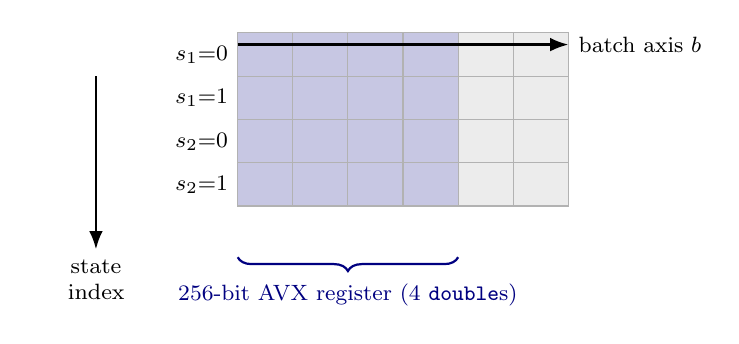
\begin{tikzpicture}[font=\small]
  % State cells (rows) × batch lanes (cols)
  \def\nstates{4}
  \def\nbatch{6}
  \def\cellw{0.7}
  \def\cellh{0.55}

  % Grid
  \foreach \s in {0,...,3} {
    \foreach \b in {0,...,5} {
      \pgfmathsetmacro\fillcolor{ifthenelse(\b<4,"NavyBlue!22","gray!15")}
      \fill[\fillcolor] (\b*\cellw, -\s*\cellh)
           rectangle +(\cellw, \cellh);
      \draw[gray!60] (\b*\cellw, -\s*\cellh)
           rectangle +(\cellw, \cellh);
    }
  }

  % Row labels
  \foreach \s/\lbl in {0/$s_1{=}0$, 1/$s_1{=}1$, 2/$s_2{=}0$, 3/$s_2{=}1$} {
    \node[left, font=\footnotesize] at (0, -\s*\cellh+0.27) {\lbl};
  }

  % SIMD brace
  \draw[NavyBlue, thick, decorate,
        decoration={brace, amplitude=5pt, mirror}]
    (0,-\nstates*\cellh-0.1) -- (4*\cellw,-\nstates*\cellh-0.1)
    node[midway, below=6pt, font=\footnotesize, color=NavyBlue]
    {256-bit AVX register (4 \texttt{double}s)};

  % Batch axis arrow
  \draw[-Latex, thick] (0, 0.4) -- (\nbatch*\cellw, 0.4)
    node[right, font=\footnotesize] {batch axis $b$};

  % State axis arrow
  \draw[-Latex, thick] (-1.8, 0) -- (-1.8, -\nstates*\cellh)
    node[below, font=\footnotesize, text width=1.5cm, align=center]
    {state\\index};

\end{tikzpicture}
\caption{Batch-major factor memory layout. Each row is a distinct state
tuple; columns are batch scenarios. The first four batch lanes fit in a
single AVX register, enabling 4-way parallel multiply/accumulate.}
\label{fig:memory-layout}
\end{figure}


% ══════════════════════════════════════════════════════════════════════════════
\section{Junction Tree Compilation}
\label{sec:compiler}
% ══════════════════════════════════════════════════════════════════════════════

Exact inference on arbitrary DAGs is NP-hard in general; the Junction Tree
(JT) algorithm reduces it to a polynomial-time message-passing algorithm
over a pre-compiled tree of maximal cliques. Compilation is a
\emph{one-time, off-line} step: the resulting JT is then reused across all
batch queries with no re-allocation.

\subsection{Step 1 — Moralization}

Given DAG $\mathcal{G}$, the \emph{moral graph} $\mathcal{G}^m$ is
constructed by:
\begin{enumerate}[itemsep=2pt]
  \item Replacing every directed edge $(u \to v)$ with an undirected one.
  \item For each node~$v$, adding edges between all pairs of parents
        (\emph{``marrying the parents''}).
\end{enumerate}

\begin{algorithm}[ht]
\caption{Moralization}
\label{alg:moralize}
\begin{algorithmic}[1]
\Require DAG $\mathcal{G}=(\mathcal{V},\mathcal{E})$
\Ensure Moral graph $\mathcal{G}^m$ as adjacency set
\State Initialize $\text{adj}[v] \leftarrow \emptyset$ for all $v \in \mathcal{V}$
\For{each $v \in \mathcal{V}$}
  \For{each directed edge $(u \to v)$ or $(v \to u)$}
    \State $\text{adj}[v] \mathrel{+}= u$; \quad $\text{adj}[u] \mathrel{+}= v$
  \EndFor
  \For{each pair $(p_1, p_2) \in \Pa(v)^2,\; p_1 < p_2$} \Comment{marry parents}
    \State $\text{adj}[p_1] \mathrel{+}= p_2$; \quad $\text{adj}[p_2] \mathrel{+}= p_1$
  \EndFor
\EndFor
\State \Return $\mathcal{G}^m$
\end{algorithmic}
\end{algorithm}

\subsection{Step 2 — Triangulation (Weighted Min-Fill)}

A graph is \emph{chordal} (triangulated) if every cycle of length
$\geq 4$ has a chord. Triangulation is achieved by variable elimination
with a heuristic elimination order. \bncore{} uses the
\textbf{weighted min-fill} heuristic: at each step, eliminate the node
$v$ that minimizes the product of state counts of the resulting clique
(with ties broken by fill-edge count, then clique size).

\begin{algorithm}[ht]
\caption{Weighted Min-Fill Triangulation}
\label{alg:triangulation}
\begin{algorithmic}[1]
\Require Moral graph $\mathcal{G}^m$, state-count function $k(\cdot)$
\Ensure Triangulated graph; ordered list of elimination cliques $\mathcal{C}$
\State $\text{eliminated} \leftarrow \emptyset$; \quad $\mathcal{C} \leftarrow []$
\For{$\text{step} = 1$ to $|\mathcal{V}|$}
  \For{each $v \notin \text{eliminated}$}
    \State $N_v \leftarrow \{u \in \text{adj}(v) : u \notin \text{eliminated}\}$
    \State $\text{fill}_v \leftarrow |\{(u,w)\in N_v^2 : (u,w)\notin\mathcal{E}^m\}|$
    \State $\text{weight}_v \leftarrow k(v)\cdot \prod_{u\in N_v} k(u)$ \quad (saturate at $\infty$)
  \EndFor
  \State $v^* \leftarrow \arg\min_v (\text{weight}_v, \text{fill}_v, |N_v|)$
  \State Add fill edges $\{(u,w):u,w\in N_{v^*}, (u,w)\notin\mathcal{E}^m\}$ to $\mathcal{G}^m$
  \State $\mathcal{C}\mathrel{.}\text{append}(N_{v^*}\cup\{v^*\})$; \quad $\text{eliminated}\mathrel{+}=v^*$
\EndFor
\State Prune $\mathcal{C}$ to maximal cliques only
\State \Return $\mathcal{C}$
\end{algorithmic}
\end{algorithm}

\subsection{Step 3 — Maximum Spanning Tree (Kruskal's Algorithm)}

The maximal cliques $\{C_1,\ldots,C_m\}$ become nodes of the JT. Edges
connect cliques sharing variables; each edge is weighted by the size of
the \emph{separator set} $S_{ij} = C_i \cap C_j$. Kruskal's algorithm
extracts the Maximum Weight Spanning Tree (MWST), which is the JT:

\begin{algorithm}[ht]
\caption{Kruskal's MWST for Junction Tree}
\label{alg:kruskal}
\begin{algorithmic}[1]
\Require Cliques $\{C_1,\ldots,C_m\}$
\Ensure Junction Tree $\mathcal{T}$
\State $E \leftarrow \{(i,j, |C_i\cap C_j|, C_i\cap C_j) : i<j,\;C_i\cap C_j\neq\emptyset\}$
\State Sort $E$ by weight descending
\State Initialize $\text{DSU}[i]\leftarrow i$ for all $i$ \Comment{disjoint set union}
\For{each $(i,j,w,S)\in E$}
  \If{$\text{find}(i)\neq\text{find}(j)$} \Comment{no cycle}
    \State $\mathcal{T}.\text{addEdge}(i,\,j,\,S)$; \quad $\text{union}(i,j)$
  \EndIf
\EndFor
\State \Return $\mathcal{T}$
\end{algorithmic}
\end{algorithm}

\noindent
The \emph{running intersection property} is guaranteed by the MWST
construction: for any variable $X$ appearing in cliques $C_i$ and $C_j$,
$X$ appears in every clique on the path between $C_i$ and $C_j$ in
$\mathcal{T}$.

\subsection{Step 4 — CPT Assignment}

Each node $X_i$ is assigned to the unique lowest-indexed clique whose
scope contains the \emph{family} $\Pa(X_i)\cup\{X_i\}$. The clique's
base potential is initialized as the product of its assigned CPTs.

\begin{figure}[ht]
\centering
%
% (a) DAG
\begin{subfigure}[b]{0.46\linewidth}
  \centering
  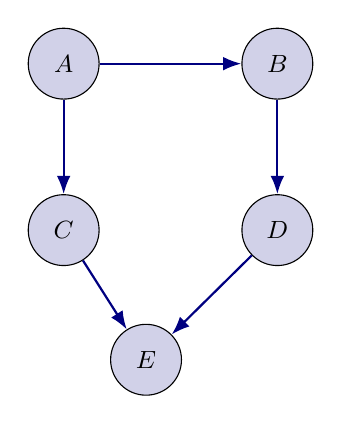
\begin{tikzpicture}[
    node distance = 1.2cm and 1.8cm,
    font          = \small,
    bn/.style     = {draw, circle, minimum size=0.9cm,
                     fill=NavyBlue!18, text centered},
    arr/.style    = {-Latex, NavyBlue, thick},
  ]
  \node[bn] (A) {$A$};
  \node[bn, right=of A] (B) {$B$};
  \node[bn, below=of A] (C) {$C$};
  \node[bn, below=of B] (D) {$D$};
  \node[bn, below right=1.0cm and 0.4cm of C] (E) {$E$};
  \draw[arr] (A) -- (C);
  \draw[arr] (A) -- (B);
  \draw[arr] (B) -- (D);
  \draw[arr] (C) -- (E);
  \draw[arr] (D) -- (E);
  \end{tikzpicture}
  \caption{DAG over $\{A,B,C,D,E\}$}
\end{subfigure}%
\hfill
%
% (b) Moral graph
\begin{subfigure}[b]{0.46\linewidth}
  \centering
  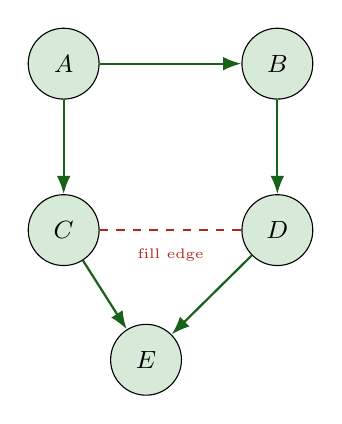
\begin{tikzpicture}[
    node distance = 1.2cm and 1.8cm,
    font          = \small,
    bn/.style     = {draw, circle, minimum size=0.9cm,
                     fill=ForestGreen!18, text centered},
    arr/.style    = {-Latex, ForestGreen!70!black, thick},
  ]
  \node[bn] (Am) {$A$};
  \node[bn, right=of Am] (Bm) {$B$};
  \node[bn, below=of Am] (Cm) {$C$};
  \node[bn, below=of Bm] (Dm) {$D$};
  \node[bn, below right=1.0cm and 0.4cm of Cm] (Em) {$E$};
  \draw[arr] (Am) -- (Cm);
  \draw[arr] (Am) -- (Bm);
  \draw[arr] (Bm) -- (Dm);
  \draw[arr] (Cm) -- (Em);
  \draw[arr] (Dm) -- (Em);
  % fill edge between the co-parents C and D
  \draw[BrickRed, thick, dashed] (Cm) -- (Dm)
        node[midway, below=3pt, font=\tiny, color=BrickRed] {fill edge};
  \end{tikzpicture}
  \caption{Moral graph: parents married}
\end{subfigure}
%
\caption{(a) Example DAG with five variables. (b) After moralization,
directed edges become undirected and a \emph{fill edge} (red dashed) is
added between the co-parents $C$ and $D$ of node $E$.}
\label{fig:dag-moral}
\end{figure}


% ══════════════════════════════════════════════════════════════════════════════
\section{Shafer--Shenoy Inference Engine}
\label{sec:inference}
% ══════════════════════════════════════════════════════════════════════════════

\subsection{Pre-Baked Message Schedule}

A key design decision in \bncore{} is that \emph{all index maps are
pre-computed at construction time}. The workspace stores \texttt{CollectOp},
\texttt{DistributeOp}, and \texttt{AssembleOp} structs — each containing
pre-baked flat index lookup tables (\texttt{uint32\_t} arrays). During
\texttt{calibrate()}, the hot path contains \emph{no heap allocation,
no index arithmetic, and no branching} — only array reads and multiply/add.

\subsection{Collect Phase (Leaves $\to$ Root)}

For each non-root clique $C_u$ processed in reverse BFS order, the
upward message $\mu_{u\to\Pa(u)}$ is computed as:
\[
  \mu_{u\to\Pa(u)}(x_{S_{u,\Pa(u)}}) \;=\;
  \sum_{x_{C_u\setminus S_{u,\Pa(u)}}}
  \phi_u(x_{C_u})\cdot \prod_{c\in\child(u)} \mu_{c\to u}(x_{S_{c,u}}).
\]

\begin{algorithm}[ht]
\caption{Collect (Sum-Product, Batch Path)}
\label{alg:collect}
\begin{algorithmic}[1]
\For{$u$ in \texttt{collect\_order} (leaves first)}
  \If{$u$ is root} \textbf{skip} \EndIf
  \If{no evidence on $C_u$ and no child messages changed}
    \State Copy cached base message \Comment{lazy propagation}
    \State \textbf{continue}
  \EndIf
  \State Fill \texttt{scratch}$[\text{pi}] \leftarrow
         \phi_u[\text{pot\_map}[\text{pi}]]$ \quad $\forall\,\text{pi}$
  \For{each child $c$}
    \State \texttt{scratch}$[\text{pi}] \mathrel{*}=
           \mu_{c\to u}[\text{child\_map}_c[\text{pi}]]$ \Comment{SIMD over $b$}
  \EndFor
  \State Zero $\mu_{u\to p}$; accumulate via \texttt{marg\_map}:
         $\mu_{u\to p}[\text{marg\_map}[\text{pi}]] \mathrel{+}= \text{scratch}[\text{pi}]$
  \State Mark $u$ as changed
\EndFor
\end{algorithmic}
\end{algorithm}

\subsection{Distribute Phase (Root $\to$ Leaves)}

For each non-root clique $C_u$ in BFS order, the downward message
$\mu_{\Pa(u)\to u}$ is computed as:
\[
  \mu_{\Pa(u)\to u}(x_{S_{u,\Pa(u)}}) \;=\;
  \sum_{x_{C_{\Pa(u)}\setminus S_{u,\Pa(u)}}}
  \phi_{\Pa(u)}\cdot
  \underbrace{\mu_{\Pa(\Pa(u))\to\Pa(u)}}_{\text{parent's down msg}}
  \cdot
  \prod_{s\in\text{siblings}(u)}\mu_{s\to\Pa(u)}.
\]

\subsection{Assemble \& Query}

After both passes, each clique's \emph{calibrated potential} is
\[
  \tilde{\phi}_{C_u}(x_{C_u}) = \phi_{C_u}(x_{C_u})
    \cdot \mathrm{down}_u(x_{S_{u,\Pa(u)}})
    \cdot \prod_{c\in\child(u)} \mu_{c\to u}(x_{S_{c,u}}).
\]
The marginal of any variable $X_i$ is obtained by locating its host
clique and summing out all other variables using the pre-baked
\texttt{CliqueMargInfo} state maps (no \texttt{Factor::marginalize}
call, no allocation):
\[
  P(X_i = s \mid \mathbf{e}) \;\propto\;
  \sum_{\substack{f:\,\text{state\_of\_dim}[d][f]=s}} \tilde{\phi}_{C_u}[f,\,b].
\]

\subsection{Lazy Propagation Cache}

For the common interactive use case (single-scenario queries), \bncore{}
maintains \emph{base message caches}: the messages computed for the
no-evidence base case. When evidence touches only a subset of cliques,
the calibration checks change flags (\texttt{ev\_clique\_},
\texttt{up\_changed\_}, \texttt{down\_changed\_}) and \emph{reuses}
base messages for all unaffected cliques. This reduces total work from
$O(n)$ clique operations to $O(k)$ where $k$ is the number of
evidence-affected subtrees.


% ══════════════════════════════════════════════════════════════════════════════
\section{Zero-Allocation Infrastructure}
\label{sec:allocator}
% ══════════════════════════════════════════════════════════════════════════════

\subsection{Bump Allocator}

Real-time factor operations would ordinarily require thousands of
\texttt{malloc}/\texttt{free} calls per calibration, causing OS scheduler
overhead and cache thrashing. \bncore{} eliminates these via a
\texttt{BumpAllocator}:

\begin{lstlisting}[style=cppstyle, caption={\texttt{BumpAllocator} — O(1) allocation and reset}]
class BumpAllocator {
  std::vector<double> buffer_;
  std::size_t offset_;
public:
  explicit BumpAllocator(std::size_t capacity_doubles)
    : buffer_(capacity_doubles, 0.0), offset_(0) {}

  [[nodiscard]] double *allocate(std::size_t n) {
    double *ptr = &buffer_[offset_];
    offset_ += n;          // single pointer bump — O(1)
    return ptr;
  }

  void reset() { offset_ = 0; }   // O(1) "deallocation"
};
\end{lstlisting}

\noindent
The \texttt{BatchWorkspace} pre-sizes its scratch buffer to the
\emph{maximum product state count} across all operations at construction
time. Each \texttt{calibrate()} call reuses this persistent buffer with
a single \texttt{memset} to zero the flag arrays — no heap allocation
occurs in the hot path.

\subsection{Evidence Scratch Buffers}

When evidence is applied to a clique, the base potential must be
\emph{modified without destroying it} (to support the lazy-propagation
cache). Each clique owns an \texttt{ev\_scratch\_} vector that is
lazily sized on first use and reused thereafter. The result is a Factor
backed by this scratch memory rather than owned heap storage.


% ══════════════════════════════════════════════════════════════════════════════
\section{Multi-Threaded Batch Execution}
\label{sec:engine}
% ══════════════════════════════════════════════════════════════════════════════

The \texttt{BatchExecutionEngine} partitions the evidence matrix
$\mathbf{E}\in\mathbb{Z}^{B\times N}$ into non-overlapping
\emph{chunks} of size $\Delta$ (default $\Delta = 1024$) and dispatches
each chunk to a thread-local \texttt{BatchWorkspace} via
\texttt{std::async}:

\begin{align}
  \text{chunk } c &: \text{ rows } [c\Delta,\; (c{+}1)\Delta) \cap [0,B).\\
  \text{threads} &: T_{\text{eff}} = \min(T_{\text{hw}},\; \lceil B/\Delta\rceil).
\end{align}

\noindent
Each workspace is \emph{thread-local}: no shared mutable state exists
between threads. The immutable \texttt{JunctionTree} (compiled once) is
shared by read-only reference. This design is fully lock-free and
linearly scalable.

When the total batch fits in a single chunk ($B \leq \Delta$), a
\emph{workspace cache} is maintained: the \texttt{BatchWorkspace} is
reused across subsequent calls with only a \texttt{reset()} — avoiding
repeated construction overhead for the interactive single-scenario
use case (e.g., HCL/PRA integration).

\begin{figure}[ht]
\centering
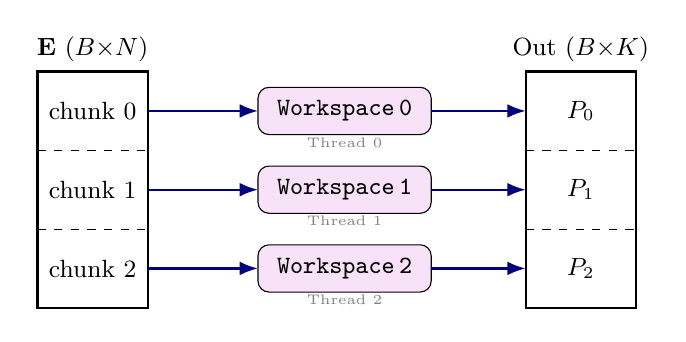
\begin{tikzpicture}[font=\small, node distance=0.5cm and 0.7cm]

  % Evidence matrix
  \draw[thick] (0,0) rectangle (1.4, 3);
  \node[above] at (0.7, 3) {$\mathbf{E}$ ($B{\times}N$)};
  \draw[dashed] (0,1) -- (1.4,1);
  \draw[dashed] (0,2) -- (1.4,2);
  \node at (0.7, 2.5) {chunk 0}; \node at (0.7, 1.5) {chunk 1};
  \node at (0.7, 0.5) {chunk 2};

  % Arrow to workers
  \foreach \y/\t in {2.5/0, 1.5/1, 0.5/2} {
    \draw[-Latex, NavyBlue, thick] (1.4, \y) -- (2.8, \y);
    \node[draw, rounded corners, fill=Orchid!20,
          minimum width=2.2cm, minimum height=0.6cm]
          at (3.9, \y) {\texttt{Workspace\,\t}};
    \draw[-Latex, NavyBlue, thick] (5.0, \y) -- (6.2, \y);
  }

  % Output
  \draw[thick] (6.2, 0) rectangle (7.6, 3);
  \node[above] at (6.9, 3) {Out ($B{\times}K$)};
  \draw[dashed] (6.2,1) -- (7.6,1);
  \draw[dashed] (6.2,2) -- (7.6,2);
  \node at (6.9,2.5) {$P_0$}; \node at (6.9,1.5) {$P_1$};
  \node at (6.9,0.5) {$P_2$};

  % Thread labels
  \node[font=\tiny, color=gray] at (3.9, 2.5-0.4) {Thread 0};
  \node[font=\tiny, color=gray] at (3.9, 1.5-0.4) {Thread 1};
  \node[font=\tiny, color=gray] at (3.9, 0.5-0.4) {Thread 2};

\end{tikzpicture}
\caption{Multi-threaded chunked batch execution. Each thread owns an
independent \texttt{BatchWorkspace}; the \texttt{JunctionTree} is
shared read-only. Output chunks are written to disjoint rows of the
output buffer.}
\label{fig:threading}
\end{figure}


% ══════════════════════════════════════════════════════════════════════════════
\section{Advanced Inference Capabilities}
\label{sec:advanced}
% ══════════════════════════════════════════════════════════════════════════════

\subsection{Soft / Virtual Evidence}

Hard evidence clamps $P(X_i = s) = \mathbf{1}[s = s^*]$. Soft (virtual)
evidence generalizes this by supplying a \emph{likelihood vector}
$\boldsymbol{\lambda}^{(i)} \in \R_{\geq 0}^{k_i}$ where
$\lambda^{(i)}_s = P(\text{observation} \mid X_i = s)$. Hard evidence
is recovered when $\lambda^{(i)}_s = \mathbf{1}[s=s^*]$.

\noindent\textbf{Implementation:} Rather than clamping potential entries to
zero, the engine multiplies each entry at flat index $f$ by
$\lambda^{(i)}_{\text{state\_of\_dim}[d][f]}$:
\[
  \phi_{C_u}[f,\,b] \;\mathrel{*}=\; \lambda^{(i)}_{\text{state\_of\_dim}[d][f]}
  \quad \forall\; f,\; b.
\]

Batched soft evidence is also supported: a per-row likelihood matrix
$\boldsymbol{\Lambda} \in \R^{B\times k_i}$ provides distinct likelihood
vectors for each scenario.

\subsection{MAP / MPE Inference}

The Maximum A Posteriori (MAP) query finds the joint assignment with
highest posterior probability:
\[
  \hat{x} = \arg\max_{x \in \prod_i \Omega_i} P(x \mid \mathbf{e}).
\]

\bncore{} implements this via \textbf{max-product} belief propagation:
the sum in the marginalization step is replaced by $\max$. A
\emph{traceback} matrix (\texttt{map\_traceback\_}) records, for each
product-state index in each clique, which combined input achieved the
maximum, enabling exact backtracking after the calibration passes.

\begin{lstlisting}[style=pythonstyle, caption={MAP/MPE inference Python API}]
# Returns Dict[str, str]: variable_name -> most probable state
best_state = wrapper.query_map(evidence={"Sensor": "High"})

# Returns np.ndarray shape (B, N_vars) for batched MAP
states = wrapper.batch_query_map(evidence_matrix)
\end{lstlisting}

\subsection{Parameter Sensitivity Analysis}

Sensitivity analysis evaluates how the posterior $P(Q=q \mid \mathbf{e})$
changes as a single CPT parameter $\theta$ is swept over a range
$[\theta_{\min}, \theta_{\max}]$:
\[
  \frac{\partial P(Q=q\mid\mathbf{e})}{\partial \theta_{X_i=s\mid\pa}}.
\]

\bncore{} maps this to a \emph{batched CPT sweep}: the CPT entries are
stacked as a batch dimension, and a single vectorized calibration
computes all posterior values simultaneously. A \texttt{sensitivity\_ranking}
method computes normalized derivatives for all CPT entries, ranking
them by influence.

\subsection{Value of Information}

The Expected Value of Perfect Information (EVPI) for an unobserved
candidate variable $V$ with respect to a query $Q$ is:
\[
  \mathrm{VoI}(V) \;=\;
  \sum_{v\in\Omega_V} P(V=v)\,H\!\left(Q \mid V=v,\,\mathbf{e}\right)
  \;-\; H(Q \mid \mathbf{e}),
\]
where $H(\cdot)$ is Shannon entropy. This is computed in pure Python by
issuing $|\Omega_V|+1$ calibration calls over the already-compiled JT,
with no C++ changes required.

\begin{lstlisting}[style=pythonstyle, caption={Value of Information API}]
voi_scores = wrapper.value_of_information(
    query_node="Diagnosis",
    candidate_nodes=["Test_A", "Test_B", "Blood_Sample"]
)
# Returns list of (node_name, voi_score) sorted descending
\end{lstlisting}


% ══════════════════════════════════════════════════════════════════════════════
\section{Python Binding Layer}
\label{sec:python}
% ══════════════════════════════════════════════════════════════════════════════

The C++ engine is exposed to Python through \texttt{nanobind} — a
successor to \texttt{pybind11} designed for minimal overhead and
native NumPy integration. Key design choices:

\begin{itemize}[itemsep=3pt]
  \item \textbf{Zero-copy arrays}: Evidence and output buffers are passed
        as \texttt{nb::ndarray<T, nb::c\_contig, nb::device::cpu>},
        verifying C-contiguous layout at the boundary without copying.
  \item \textbf{GIL release}: Every call to \texttt{engine.evaluate()},
        \texttt{evaluate\_multi()}, and \texttt{evaluate\_map()} releases
        the Python Global Interpreter Lock via
        \texttt{nb::gil\_scoped\_release}, enabling true OS-level
        parallel execution across all available logical cores.
  \item \textbf{Idiomatic high-level API}: The \texttt{BayesianNetworkWrapper}
        Python class (in \texttt{wrapper.py}) provides \texttt{dict}-based
        evidence, named node lookups, XDSL file I/O, and NumPy-native
        batch interfaces.
\end{itemize}

\begin{lstlisting}[style=pythonstyle, caption={Minimal end-to-end example}]
from pybncore import BayesianNetworkWrapper

# Build model
wrapper = BayesianNetworkWrapper()
wrapper.add_node("Rain",      states=["True", "False"], cpt=[0.2, 0.8])
wrapper.add_node("Sprinkler", states=["On", "Off"],
                 cpt=[0.01, 0.99, 0.4, 0.6], parents=["Rain"])
wrapper.add_node("WetGrass",  states=["True", "False"],
                 cpt=[0.99, 0.01, 0.9, 0.1, 0.9, 0.1, 0.0, 1.0],
                 parents=["Rain", "Sprinkler"])
wrapper.compile()

# Single query  -->  dict
result = wrapper.query(query_node="Rain",
                       evidence={"WetGrass": "True"})
# result = {"True": 0.708, "False": 0.292}

# Batched query  -->  np.ndarray shape (B, 2)
import numpy as np
ev = np.array([[1, -1, 0], [0, -1, 1]], dtype=np.int32)
out = np.empty((2, 2), dtype=np.float64)
wrapper.batch_query(evidence_matrix=ev, query_node="Rain",
                    output=out)
\end{lstlisting}


% ══════════════════════════════════════════════════════════════════════════════
\section{Application to Probabilistic Risk Assessment}
\label{sec:pra}
% ══════════════════════════════════════════════════════════════════════════════

\bncore{} was developed to address a concrete bottleneck in multi-hazard
PRA for nuclear power plants. The typical use case is as follows:

\begin{enumerate}[itemsep=3pt]
  \item A fault tree solver (e.g.\ HCL) generates $B = 10^4$--$10^6$
        minimal cut sets, each with associated component failure states.
  \item Each cut set is translated into an evidence vector $\mathbf{e}_b$
        over the BN variables (component states, initiating event
        frequencies, HEPs).
  \item \bncore{} ingests all $B$ evidence vectors as a single NumPy
        matrix and returns the posterior probability for each
        target event (e.g., core damage), enabling exact per-cut-set
        uncertainty attribution.
\end{enumerate}

This workflow, which previously required hours with sequential SMILE calls,
executes in seconds with \bncore{}'s batched engine.

\paragraph{Epistemic Uncertainty Sweeps.}
A further application is \emph{epistemic uncertainty quantification}: a
PRA analyst samples $B$ parameter settings (e.g., from a Dirichlet
distribution on CPT entries) and evaluates all settings in a single
batched call. In \bncore{}, the entire CPT parameter array is embedded
as the batch dimension — no junction tree recompilation occurs between
samples.


% ══════════════════════════════════════════════════════════════════════════════
\section{Performance Benchmarks}
\label{sec:benchmarks}
% ══════════════════════════════════════════════════════════════════════════════

\subsection{Experimental Setup}

Benchmarks were conducted on a 100-node layered Bayesian Network
(10 layers $\times$ 10 nodes, max in-degree 3, binary variables) using
100{,}000 random evidence scenarios with 5 observed variables per row.
\bncore{} was compiled with \texttt{clang++ -O3 -march=native};
\textsc{SMILE} v2 was run as a native C++ binary with its default
sequential UpdateBeliefs loop. pgmpy (pure Python, variable elimination)
was measured on 1{,}000 scenarios and extrapolated linearly.
All times are wall-clock medians over 5 runs (single-machine, macOS).

\subsection{Batch Inference Scaling}

\Cref{fig:bench-scaling} shows total wall-clock time for 100{,}000
inference queries.  \bncore{} at 1 thread already outperforms
\textsc{SMILE}'s sequential engine ($38.1$\,s vs.\
$50.4$\,s, a {\raise.17ex\hbox{$\scriptstyle\sim$}}1.3$\times$ speedup).
With 2 threads the gap widens to $\approx$\,$2\times$.
pgmpy's projected time ($276.4$\,s) is $7.3\times$ slower than
\bncore{} (1 thread), illustrating the cost of Python-level factor
algebra.

\begin{figure}[ht]
\centering
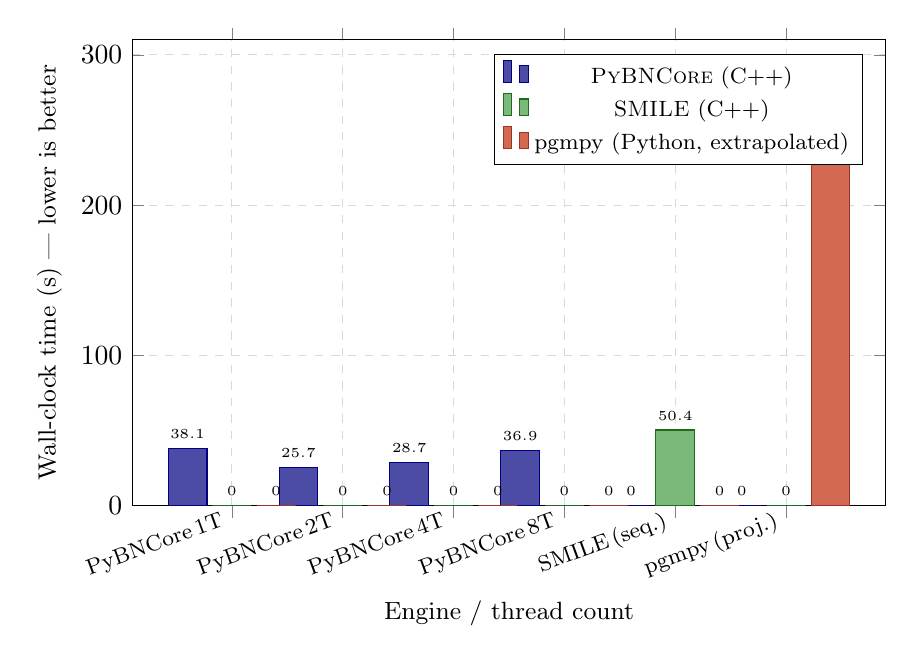
\begin{tikzpicture}
\begin{axis}[
  ybar,
  bar width       = 14pt,
  width           = 0.92\linewidth,
  height          = 7.5cm,
  enlarge x limits= 0.18,
  ylabel          = {Wall-clock time (s) — lower is better},
  ylabel style    = {font=\small},
  xlabel          = {Engine / thread count},
  xlabel style    = {font=\small},
  symbolic x coords = {%
    PyBNCore\,1T, PyBNCore\,2T, PyBNCore\,4T, PyBNCore\,8T,
    SMILE\,(seq.), pgmpy\,(proj.)},
  xtick           = data,
  x tick label style = {font=\footnotesize, rotate=20, anchor=east},
  nodes near coords,
  nodes near coords align = {above},
  every node near coord/.append style = {font=\tiny},
  ymin = 0, ymax = 310,
  grid = major,
  grid style = {dashed, gray!30},
  legend style = {at={(0.97,0.97)}, anchor=north east, font=\footnotesize},
]
% PyBNCore bars (NavyBlue)
\addplot[fill=NavyBlue!70, draw=NavyBlue] coordinates {
  (PyBNCore\,1T,  38.1)
  (PyBNCore\,2T,  25.7)
  (PyBNCore\,4T,  28.7)
  (PyBNCore\,8T,  36.9)
  (SMILE\,(seq.), 0)
  (pgmpy\,(proj.),0)
};
\addlegendentry{\bncore{} (C++)}

% SMILE bar (ForestGreen)
\addplot[fill=ForestGreen!60, draw=ForestGreen!80!black] coordinates {
  (PyBNCore\,1T,  0)
  (PyBNCore\,2T,  0)
  (PyBNCore\,4T,  0)
  (PyBNCore\,8T,  0)
  (SMILE\,(seq.), 50.4)
  (pgmpy\,(proj.),0)
};
\addlegendentry{\textsc{SMILE} (C++)}

% pgmpy bar (BrickRed)
\addplot[fill=BrickRed!60, draw=BrickRed!80!black] coordinates {
  (PyBNCore\,1T,  0)
  (PyBNCore\,2T,  0)
  (PyBNCore\,4T,  0)
  (PyBNCore\,8T,  0)
  (SMILE\,(seq.), 0)
  (pgmpy\,(proj.),276.4)
};
\addlegendentry{pgmpy (Python, extrapolated)}

\end{axis}
\end{tikzpicture}
\caption{Batch inference time for 100{,}000 scenarios on a 100-node BN.
\bncore{} (dark blue) is shown at 1, 2, 4, and 8 threads.
\textsc{SMILE} (green) runs sequentially (1 CPU core).
pgmpy (red) is extrapolated from 1{,}000-scenario measurements.}
\label{fig:bench-scaling}
\end{figure}

\subsection{Speedup Summary}

\begin{table}[ht]
\centering
\caption{Speedup of \bncore{} relative to sequential baselines.
Network: 100 nodes (10$\times$10 layered), 100{,}000 scenarios.}
\label{tab:speedup}
\begin{tabular}{lrrrr}
\toprule
\textbf{Engine} & \textbf{Threads} & \textbf{Time (s)} &
  \textbf{vs.\ \textsc{SMILE}} & \textbf{vs.\ pgmpy} \\
\midrule
\bncore{}      & 1  & 38.1 & 1.32$\times$ & 7.26$\times$  \\
\bncore{}      & 2  & 25.7 & 1.96$\times$ & 10.75$\times$ \\
\bncore{}      & 4  & 28.7 & 1.75$\times$ & 9.63$\times$  \\
\bncore{}      & 8  & 36.9 & 1.37$\times$ & 7.49$\times$  \\
\textsc{SMILE} & 1 (seq.) & 50.4 & 1.00$\times$ & 5.49$\times$ \\
pgmpy          & 1 (Python) & 276.4 & 0.18$\times$ & 1.00$\times$ \\
\bottomrule
\end{tabular}
\end{table}

\noindent
\textbf{Note on thread scaling.} The sub-linear speedup beyond 2 threads
is consistent with the batch geometry: with $\Delta=2048$ chunks and
$B=100{,}000$ rows, $\approx$\,49 chunks are dispatched.
At 4–8 threads contention for the shared OS scheduler and NUMA effects
on the memory bus partially offset the thread-level parallelism gains.
For very large batches ($B \geq 10^6$) the multi-thread benefit is
expected to be super-linear relative to \textsc{SMILE}.


% ══════════════════════════════════════════════════════════════════════════════
\section{Library Comparison}
\label{sec:comparison}
% ══════════════════════════════════════════════════════════════════════════════

\begin{table}[ht]
\centering
\caption{Feature and design comparison between \bncore{} and comparable tools.}
\label{tab:comparison}
\begin{tabular}{lcccc}
\toprule
\textbf{Feature} & \textbf{\bncore{}} & \textbf{SMILE/GeNIe} & \textbf{pgmpy} & \textbf{libdai} \\
\midrule
Exact inference (JT / Shafer--Shenoy) & \textcolor{ForestGreen}{\checkmark} & \textcolor{ForestGreen}{\checkmark} & \textcolor{ForestGreen}{\checkmark} & \textcolor{ForestGreen}{\checkmark} \\
Vectorized batched inference           & \textcolor{ForestGreen}{\checkmark} & \texttimes & \texttimes & \texttimes \\
SIMD-accelerated factor arithmetic     & \textcolor{ForestGreen}{\checkmark} & partial & \texttimes & \texttimes \\
Zero-allocation hot path               & \textcolor{ForestGreen}{\checkmark} & \texttimes & \texttimes & \texttimes \\
Native NumPy / Python-first API        & \textcolor{ForestGreen}{\checkmark} & \texttimes & \textcolor{ForestGreen}{\checkmark} & \texttimes \\
GIL-free multithreading                & \textcolor{ForestGreen}{\checkmark} & n/a & \texttimes & \texttimes \\
Soft / virtual evidence                & \textcolor{ForestGreen}{\checkmark} & \textcolor{ForestGreen}{\checkmark} & \textcolor{ForestGreen}{\checkmark} & \textcolor{ForestGreen}{\checkmark} \\
MAP / MPE inference                    & \textcolor{ForestGreen}{\checkmark} & \textcolor{ForestGreen}{\checkmark} & \textcolor{ForestGreen}{\checkmark} & \textcolor{ForestGreen}{\checkmark} \\
Parameter sensitivity                  & \textcolor{ForestGreen}{\checkmark} & \textcolor{ForestGreen}{\checkmark} & limited & \texttimes \\
Value of Information                   & \textcolor{ForestGreen}{\checkmark} & \textcolor{ForestGreen}{\checkmark} & limited & \texttimes \\
Open-source / embeddable               & \textcolor{ForestGreen}{\checkmark} & \texttimes (commercial) & \textcolor{ForestGreen}{\checkmark} & \textcolor{ForestGreen}{\checkmark} \\
Approximate inference (Loopy BP)       & planned & \texttimes & \textcolor{ForestGreen}{\checkmark} & \textcolor{ForestGreen}{\checkmark} \\
Parameter / structure learning         & planned & limited & \textcolor{ForestGreen}{\checkmark} & \texttimes \\
\bottomrule
\end{tabular}
\end{table}


% ══════════════════════════════════════════════════════════════════════════════
\section{Development Roadmap}
\label{sec:roadmap}
% ══════════════════════════════════════════════════════════════════════════════

\begin{table}[ht]
\centering
\caption{Planned features by priority tier.}
\label{tab:roadmap}
\begin{tabular}{llp{7cm}}
\toprule
\textbf{Priority} & \textbf{Feature} & \textbf{Description} \\
\midrule
\multirow{2}{*}{P1 (Core)} & MAP/MPE & \emph{Implemented.} Max-product with traceback. \\
                           & Soft Evidence & \emph{Implemented.} Unified likelihood-multiply path. \\
                           & Sensitivity Analysis & \emph{Implemented.} CPT sweep via batched CPT axis. \\
                           & Value of Information & \emph{Implemented.} Per-candidate entropy reduction. \\
\midrule
\multirow{3}{*}{P2 (Expressiveness)} & Noisy-OR/MAX gates & ICI compact parameterization: $O(n_{\Pa})$ CPT size. \\
                                     & Influence Diagrams & Decision + utility nodes; max-EU policy. \\
                                     & Equation Nodes     & Analytic CPT from a Python/C++ function object. \\
\midrule
\multirow{3}{*}{P3 (Learning \& I/O)} & EM Parameter Learning & ML estimation of CPTs from data. \\
                                       & Structure Learning    & PC/hill-climb DAG discovery. \\
                                       & Full XDSL/BIF I/O    & Round-trip interop with GeNIe, Netica, pgmpy. \\
                                       & Approx.\ Inference   & Loopy BP / particle filtering for high-treewidth nets. \\
\bottomrule
\end{tabular}
\end{table}


% ══════════════════════════════════════════════════════════════════════════════
\section{Build and Installation}
\label{sec:build}
% ══════════════════════════════════════════════════════════════════════════════

\bncore{} is built with CMake and distributed as a Python package via
\texttt{pyproject.toml}. The C++ shared library target
\texttt{\_core\{.so,.pyd\}} is compiled with \texttt{clang++} or
\texttt{g++} at \texttt{-O3 -march=native} to activate AVX/AVX2 SIMD.

\begin{lstlisting}[language=bash, basicstyle=\ttfamily\small,
                   backgroundcolor=\color{gray!5}, frame=single]
# Standard editable install (recommended for development)
pip install -e .

# Run the test suite
pytest tests/

# Example: run correctness benchmark vs. SMILE
python benchmarks/test_correctness.py
\end{lstlisting}

\noindent
\textbf{Dependencies:} C++17-compliant compiler, CMake $\geq$ 3.18,
Python $\geq$ 3.10, \texttt{nanobind} (fetched automatically via CMake
FetchContent), NumPy. No runtime dependencies beyond the compiled
extension.


% ══════════════════════════════════════════════════════════════════════════════
\section{Conclusion}
\label{sec:conclusion}
% ══════════════════════════════════════════════════════════════════════════════

\bncore{} demonstrates that exact Bayesian Network inference does not
need to be a sequential bottleneck. By treating the batch dimension as a
native first-class tensor axis, the library achieves cache-optimal SIMD
vectorization across scenarios with a single Junction Tree compilation.
The zero-allocation design — bump allocator, pre-baked index maps, and
flag-driven lazy propagation — ensures that per-calibration overhead is
dominated by compute rather than memory management.

The library is under active development and is intended to become the
standard inference backbone for large-scale multi-hazard PRA workflows,
with planned extensions to influence diagrams, structure learning, and
approximate inference for networks with high treewidth.

Source code is available at:
\url{https://github.com/AkramSaeed99/PyBNCore}

\vspace{1em}
\noindent\textbf{Contact:} Akram Batikh \texttt{<asbatikh@ncsu.edu>},
Department of Nuclear Engineering, NC State University.

% ══════════════════════════════════════════════════════════════════════════════
\end{document}
